\documentclass[11pt]{article}
\usepackage{amsfonts}
\usepackage{amsmath}
\usepackage[makeroom]{cancel}
\usepackage[top=.5in, bottom=1in, left=.5in, right=.5in]{geometry}
\fontsize{15}{2} 
\allowdisplaybreaks[1]
\usepackage{setspace}
\onehalfspacing
\usepackage{listings}
\usepackage{hyperref}
\usepackage{marvosym}
\usepackage{courier}
\usepackage{graphicx} % more modern
\usepackage{subfigure} 
\usepackage{caption}
\usepackage{listings}
\def\etal{{\textit{et~al.~}}}

\begin{document}

\vspace*{8cm}

\centerline{\sc \Large Machine Learning and Computational Statistics: Project Report}

\vspace{1cm}

\centerline{\sc \small Emily Denton (eld297)  \& Rahul Gopalkrishnan (rg2451)}
         
\clearpage 


\section{Introduction}
Neural network based models for computing continuous vector representations of words have gained popularity. 
In particular, Mikolov \etal \cite{mikolov1, mikolov2} have proposed two new models, called the Continous Bag-of-Words (CBOW) model and the Skip-gram model, for learning a continuous embedding space for words from raw text data. Such representations are useful as inputs to NLP applications since the embedding space learned may contain many interesting properties. Recent work\etal \cite{mikolov3} showed that the embedding space learned from these models has an interesting linear structure that can be exploited to finding analogical relationships between words. They show that analogical questions of the form `King is to man as Queen is to \_\_\_\_' can be solved by algebraic operations on the word vectors. In this case, they compute the vector (King - man + Queen) and then search for its nearest word vector. The result should be woman. This could potentially be useful in tasks such as Information Extraction where given a set of known analogies, one would like to discover new vector pairs that have a similar relationship. 

Compared to related work in learning language models\cite{bengio,mikolov5}, the neural language models are log linear, and thus have a lower computational complexity. To our knowledge, given how recent the work by Mikolov et. al. is, it is unclear if anyone has managed to successfully discover relationships automatically from a set of word vectors. Our aim is a first attempt at doing so. 

Our approach uses techniques in unsupervised learning such as clustering and SVD to analyze the structure of the word relationships. We separate our results into several sections. Since we do not have access to the amount of text data that Google possesses, we present results that attempt to quantify the effect of training data size of the quality of resulting vector representations. We investigate the differences between the CBOW and the Skip-Gram models with respect to their performance on the analogical reasoning dataset. Next, we visualize the lower-dimensional representation of the analogies to attempt to discover the underlying structure. Finally, we attempt to learn the analogies automatically.   


\section{Problem definition}

\subsection{Learning a word embedding space}

In order to learn an embedding of words into a vector space, we use the training code provided by Mikolov \etal in word2vec\cite{word2vec}. There are two different models, the Skip-Gram model and the Continuous Bag of words (CBOW) model. Both models consist of a projection layer followed by a softmax layer. They differ in the precise inputs and outputs used. The training data for both models consists of a sequence of words, $w_1, w_2, ..., w_N$. Let $M$ denote the size of the vocabulary (i.e. the number of distinct words in the entire training sequence). We described each of them in turn. 

\subsubsection{Skip Gram}
The Skip-Gram model takes a single word as input and aims to predict the surrounding words, where the order of the surrounding words matters. More specifically, we want to find the parameters $W$ which maximize the conditional log probability of the context of a given word:

\begin{align*}
	\arg \max_{W} \sum_{n=1}^{N} [\sum_{-c \leq t \leq c; t \neq n} \log p(w_{n+c} | w_n; W)]
\end{align*}
where $c$ is the size of the context window being considered (in our experiments we set c = 6). 

The output probability is given by
\begin{align*}
p(w_{O} | w_{I}; W) = \frac{ \exp \big(\phi(w_O) \cdot \phi(w_I) \big)}{\sum_{j=1}^M \exp \big(\phi(w_j) \cdot \phi(w_I) \big)}
\end{align*}


where $\phi(w_i) = W^{\top}x_i$ is the vector representation of $w_i$ (letting $x_i$ denote the 1-hot input vector for with i). The weights $W$ are learned via gradient descent. After training, the final vector representations, $\phi(w_i) \forall i$, are computed front he matrix $W$.



\subsubsection{Continuous Bag of Words (CBOW)}
Unlike the skip gram model, the continuous bag of words makes a bag of words assumption by summing up the projections of the context for a given word and trying to predict the word. More specifically, we want to find the parameters $W$ that maximize the conditional log probability of a word, given the surround words. 
\begin{equation}
	argmax_{\theta} \prod_{w\in text} p(w|k;\theta) \text{ where } k = \sum_{c \in C(w)} v_c
\end{equation}



Given a text corpus, the code provided trains a CBOW or Skip-Gram model and produces a file where every word is assigned a vector in $\mathbb{R}^n$ where we assigned $n=300$.


\begin{figure}[h]
\centering
\includegraphics[width=\textwidth]{./images/model_images.pdf}
\caption{CBOW and Skip-Gram Models. Image adopted from \cite{mikolov1}}
\label{fig:top_k}
\end{figure}

\clearpage 


\subsection{Exploring properties of learned word embedding space}


\section{Experimental results}

\subsection{Data}
The data for our experiments came from two sources. The first was a set of word vectors released by Google\cite{word2vec}. These were vectors that were trained using a skip-gram model on Google's internal dataset. We trained our own set of vectors using both the CBOW and Skip-Gram models on a corpus described below. While we did conduct experiments on the three models mentioned above, we noticed that the vectors created by Google gave better results on every section of the analogical reasoning dataset and therefore further work was done primarily using those vectors. 

\subsubsection{Training data}
The training data was created by appending several sources of text that were freely available on the web such as the English text of Wikipedia, NewsCrawl (which contains several thousands of news articles collected across the years), text8 and Europarl (which contains transcriptions of the proceedings of the European parliament).


\subsubsection{Test data}\label{sec:test_data}
Mikolov \etal \cite{mikolov3} propose evaluating the regularities of the learned embedding space with a test set of analogy questions. The questions are of the form "{\it a} is to {\it b} as {\it c} is to \_\_ ". The test set contains 14 different types of analogies (see Table \ref{table:analogical}) relating to semantic concepts and grammatical relations. 

\begin{table}[h]
\small
	\caption{Analogical reasoning test set}
	\label{table:analogical}
	\centering
    \begin{tabular}{| c |  c | c |}
    \hline
    {\bf Relation} & {\bf \# Questions} & {\bf Example} \\
    \hline
     capital-common-countries & 506 & Athens : Greece \\
     & & Bangkok : Thailand\\
     \hline
    capital-world &   4524  & Abuja : Nigeria \\
    & & Accra : Ghana\\
    \hline
    currency & 866 & Algeria : dinar\\
    & & Japan : yen\\
   \hline
   city-in-state & 2467 & Chicago : Illinois \\
   & & Houston Texas\\
   \hline
    family &  506 & brother : sister \\
    & & mother : father\\
    \hline
    adjective-to-adverb & 992 & amazing : amazingly \\
    & & calm : calmly\\
    \hline
    opposite & 813 & acceptable : unacceptable \\
    & & aware : unaware\\
    \hline
    comparative & 1331 & bad : worse \\
    & & big : bigger\\
    \hline
    superlative & 1122 & bad : worst \\
    & & big : biggest\\
    \hline
    present-participle & 1056 & code : coding\\
    & & dance : dancing\\
    \hline
    nationality-adjective & 1599 & Albania : Albanian \\
    & & Argentina : Argentinean\\
    \hline
    past-tense & 1560 & dancing : danced \\
    & & decreasing : decreased\\
    \hline
    plural & 1332 & banana : bananas \\
    & & bird birds\\
    \hline
    plural-verbs &  & eat : eats \\
    & 870 & generate : generates\\
    \hline
    \end{tabular}
\end{table}


\subsection{Results}

\subsubsection{Measuring linguistic regularity via analogies}
We evaluate the performance of (a) pre-trained Google vectors, (b) our Skip-Gram model, (c) our CBOW model, on the analogical reasoning test set introduced in section \ref{sec:test_data}. Given three query words (e.g. {\it Paris, France, London}), the task is to return the answer that fits with the analogy (in this case, {\it England}). This problem can be solved in many ways. Mikolov \etal \cite{mikolov1} propose a simple solution that relies on the inherent regularities of the embedding space learned by the Skip-Gram and CBOW models. The method uses simple vector algebra in the embedding space to find the solution word given three query words. For example, suppose the analogical relation of interest is {\it A} is to {\it B} as {\it} C is to {\it D}. Given three query words, {\it A, B, C}, the predicted solution is computed as follows:
\begin{enumerate}
\item Compute the vector representations of each word, $\phi(A), \phi(B), \phi(C)$.
\item Let $v = \phi(B) - \phi(A) + \phi(C)$.
\item Do a nearest neighbors search, based on cosine distance, to find the $k$ closest word vectors to $v$. In other words, solve for the top $k$ solutions to 
	\begin{align} \max_u 1 - \frac{ v \cdot u}{\| u \| \| v \|}\ \end{align}
\end{enumerate}

The top-$k$ accuracy is defined as the number of times $D$ appears in the set of $k$ closest words to $v$. The intuition behind this method is that the cosine distance between $\phi(A - B)$ and $\phi(C - D)$ is small when {\it A} and {\it B} are analogous to {\it C} and {\it D}. Figure \ref{fig:offsets} illustrates this intuition. 

\begin{figure}[h]
\centering
\includegraphics[width=.45\textwidth]{./images/king_queen.png}
\caption{Vector offsets for three analogous word pairs.}
\label{fig:offsets}
\end{figure}

Table \ref{tab:analogical_acc} shows the top-$k$ accuracy on the analogical reasoning dataset of the pre-trained Google vectors (GoogleVec) and the Skip-Gram and CBOW models that we trained. The Google vectors outperform both of our trained models for all $k$. This is to be expected since the Google vectors were trained on far more data than we have access to. 

Our CBOW model performs consistently worse than our Skip-Gram model. We hypothesize that this is a factor of the amount of training data we used to train our models. The CBOW model throws away a lot of information by ignoring the ordering of words. In the limit of infinite data, the bag-of-words assumption might not matter, however in a limited data setting we believe the CBOW model is hurt more than the Skip-Gram model due to the loss of information. 

Figure \ref{fig:top_k} plots the top-$k$ accuracy as a function of $k$ for the three models split up by analogy types. Figure \ref{fig:accuracy_per_question}  plots the top-5 accuracy of the three models for each of the analogy question types. A very interesting pattern emerges when we consider these results. We can break down the analogy questions into two type: (1) Analogies involving semantic relations between words such as capital-country, currency-country, and family relations (1) Grammatical analogies such as past/present tense. singular/plural terms, and present-participle relations. We notice that the Skip-Gram model performs better on analogical questions of type (2) whereas the CBOW model performs better on the questions of type (2). We hypothesize that this is a function of the number of examples of each kind of relation. The semantic analogies appear in very specific contexts. For example, the word {\it France} is unlikely to appear in general text but would rather appear in particular contexts. However, words in the grammatical relations are not specific to a particular context and would appear in a very wide variety of sentences. Thus, we hypothesize that the models have, in some sense, more information about grammatical relations than they do about specific semantic relations during training. Thus, since the CBOW model performs better when there is more data available, the CBOW model performs worse on semantic analogical relations than grammatical ones. 


\begin{table}[h]
	\caption{Top k Accuracy on Analogical Reasoning Test}
	\label{tab:analogical_acc}
	\centering
    \begin{tabular}{| c | c | c | c |}
    \hline
    \textbf{Top k} & \textbf{GoogleVec} & \textbf{CBOW} & \textbf{Skip-Gram}\\ \hline
    1 & 20.185\% & 3.029\% & 6.211\%  \\ \hline
    2 & 68.967\% & 24.764\%& 46.986\% \\ \hline
    3 & 78.346\% & 37.919\%& 59.179\% \\ \hline
    4 & 82.424\% & 43.921\%& 65.314\% \\ \hline
    5 & 84.716\% & 47.513\%& 68.967\% \\ \hline
    6 & 86.246\% & 50.332\%& 71.479\% \\ \hline
    7 & 87.285\% & 52.553\%& 73.362\% \\ \hline
    8 & 88.149\% & 54.308\%& 74.631\% \\ \hline
    9 & 88.835\% & 55.879\%& 75.716\% \\ \hline
    10 & 89.352\% & 57.142\%& 76.698\% \\ \hline
    \end{tabular}
\end{table}


\begin{figure}[h]
\centering
\includegraphics[width=\textwidth]{./images/top_k.pdf}
\caption{Top K accuracy for increasing K.}
\label{fig:top_k}
\end{figure}

\begin{figure}[h]
\centering
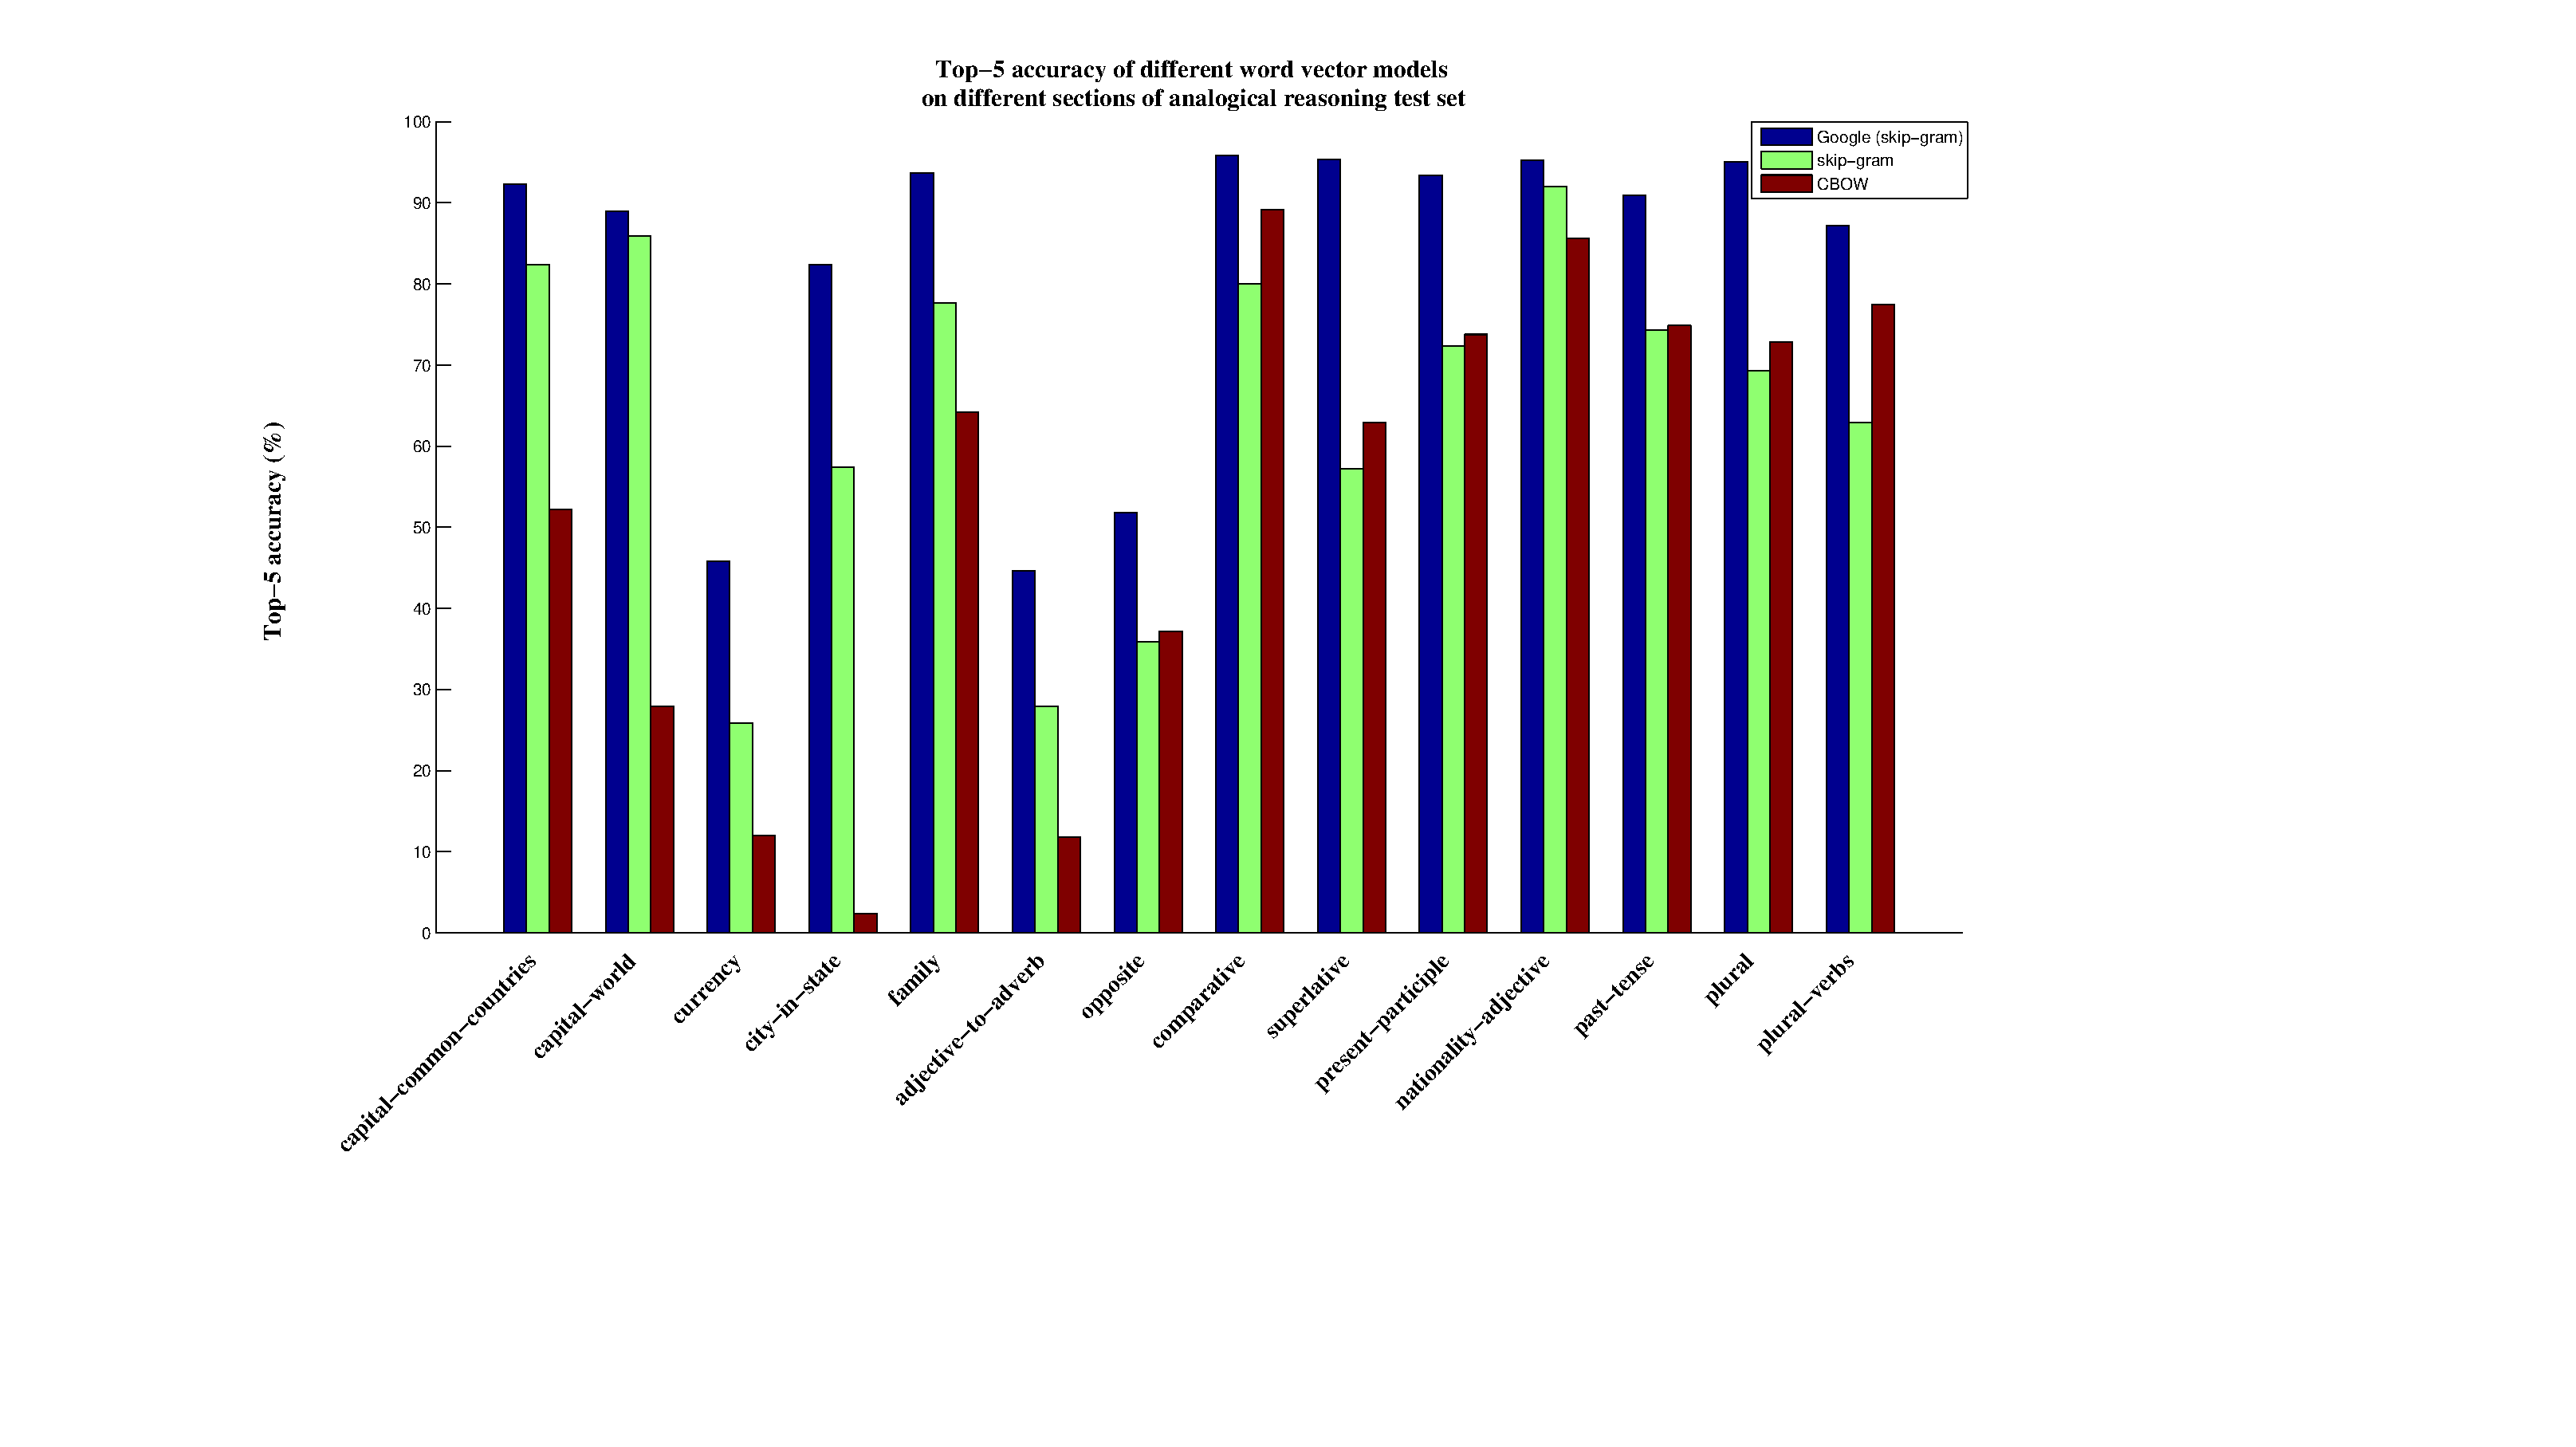
\includegraphics[width=\textwidth]{./images/analog_accuracy_per_question.eps}
\caption{Top-5 accuracy per analogy question type.}
\label{fig:accuracy_per_question}
\end{figure}


\subsubsection{Visualizing low dimensional approximations of embedding space}

We explored the low dimensional structure of different words used in the analogical reasoning set. In an attempt to gain some insight into the embedding space we did the following:
\begin{enumerate}
  \item Take 3 words from one of the quartets in the analogical reasoning test set and compute the subspace that best fits the corresponding word vectors. (For example, fine the plane that best approximates $\phi(Paris), \phi(France)$ and $\phi(London)$. 
  \item Project all word vectors onto this plane.
  \item Throw away all vectors greater than some threshold away from the plane (in the examples plotted below we kept only the closest 20 vectors).
  \item Plot the remaining word vectors projected onto the plane, coded based on Euclidean distance from the plane (the radius of the point is proportional to the distance, so larger implies farther away). 
  \item Highlight points that would be predicted (using the projected vectors) within the top $k$ (we used $k = 5$) using the vector offset method.
\end{enumerate}


\begin{figure}[t]
\centering
\subfigure[Greece : Athens - Thailand : Bangkok]{
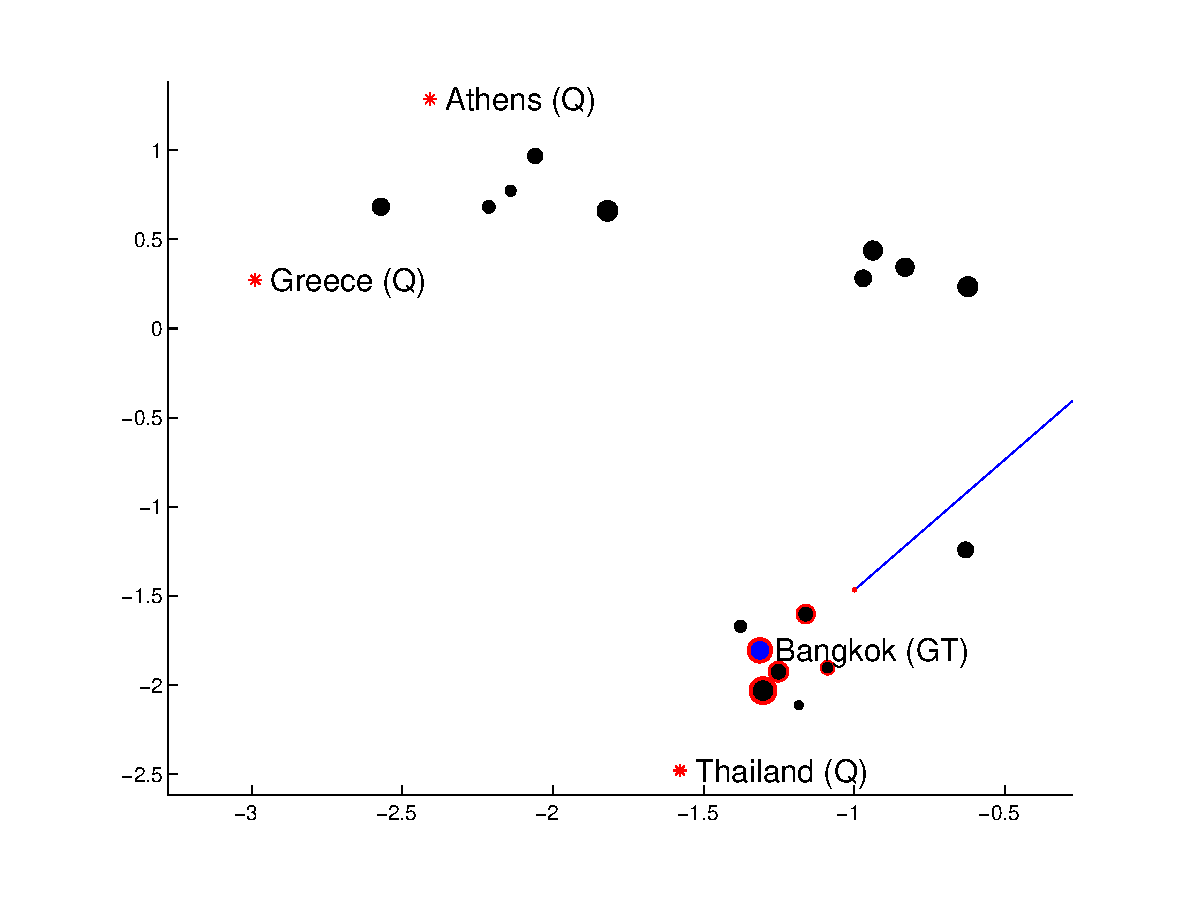
\includegraphics[width=.45\textwidth]{./images/greece_athens_thailand_bangkok.eps}
}
\subfigure[Greece : Athens - Japan : Tokyo]{
\includegraphics[width=.45\textwidth]{./images/greece_athens_japan_tokyo.eps}
}

\subfigure[Greece : Athens - Russia : Moscow]{
\includegraphics[width=.45\textwidth]{./images/greece_athens_russia_moscow.eps}
}
\subfigure[Greece : Athens - Egypt : Cairo]{
\includegraphics[width=.45\textwidth]{./images/greece_athens_egypt_cairo.eps}
}
\caption{Analogical reasoning word vectors projected onto 2D plane}
\label{fig:offsetProj}
\end{figure}

Figure \ref{fig:offsetProj} shows for of these such plots using country-capital analogies. In the plots, the red $*$'s denote the analogical query vectors, $\phi(A), \phi(B), \phi(C)$, projected onto the plane of best fit. The red $\cdot$ denotes the vector computed with the vector offset method ($\phi(B) - \phi(A) + \phi(C)$) projected onto the same plane. A blue line is drawn format he origin to this point to elucidate the direction of the vector (recall we only care about the direction of the vector, not it's magnitude). The true solution vector, $\phi(D)$, projected onto the same plane, is plotted with a blue circle. The radius of the circle indicates the distance the point lies form the plane. Finally, the black points denote the 20 closest word vectors to the plane, where again, the size of the point indicates distance front he plane. The points that would be predicted as being in the top-5 solution set are highlighted in red. Figure \ref{fig:offsetProj} (a)-(c) are examples where the correct answer is found int he top-5 (as indicated by the red circle around the blue point). Figure \ref{fig:offsetProj} (d) shows an examples where the correct word is not found in the top-5 set. This case is interesting because the true solution is very close (based on cosine distance) to ($\phi(B) - \phi(A) + \phi(C)$), however it was too far away from the plane to be found. 

One could imagine constructing a new method of answering the analogical query questions using this information by first restricting the set of possible solution vectors to only the $p$ closest ones to the plane and then doing the top-$k$ search for a solution. We tried this experiment for a variety of $k$ and $p$ and did not find it to perform better than the original method. This is to be expected given the huge amount of information that is being thrown away. However, it is interesting that the method does allow some questions to be answered correctly. We achieved a 30\% top-5 accuracy for $p = 20$, which means that a significant amount of information is retained after projecting down into 2 dimensions.  

\subsubsection{Finding analogical relations}

Our final goal was to try and uncover analogical relation automatically. Our approach to this is based on the basic insight that the cosine distance for pairs of offsets will be small if the pairs are analogous. In other words we would expect 
\begin{align}1 - \frac{(\phi(brother) - \phi(sister)) \cdot (\phi(father) - \phi(mother))}{ \| \phi(brother) - \phi(sister)) \| \| (\phi(father) - \phi(mother)\|}\end{align}
while we would expect 
 \begin{align}1 - \frac{(\phi(cat) - \phi(sister)) \cdot (\phi(running) - \phi(Canada))}{ \| \phi(cat) - \phi(sister)) \| \| (\phi(running) - \phi(Canada)\|}\end{align} 
 to be large. 

We attempted to cluster word vector offsets based on cosine distance.We tried two methods: (1) Spectral clustering where the cosine distance between offsets is used as the affinity matrix (2) K-means there cosine distance is used as the distance metric. 

\section{Conclusion}

In conclusion, this report details our investigations into neural language models and the properties of the continuous vector representations that result from training these models. We show that having more data results in vectors whose linear properties are more amenable for use in finding analogies. We conjecture that the vast amounts of data that Google trains these models on allows the vectors to consistently outperform any models that we train when evaluated on the analogical reasoning dataset. We visualize the underlying structure of the linear properties and see that there exists some noisy linear structure in two and three dimensions. Our results from  clustering finds analogies absent in the original test set. Such a model could be used by asking which cluster a new vector offset pair fits best in. Most of our work was done using the vectors provided by Google. It would be interesting to see if we could still find interesting analogies when the models are trained with limited data. While clustering analogies does indeed let us find interesting analogies. We are currently evaluating supervised linear models to predict different kinds of analogies when given a pairs of vector offsets. 

\clearpage

\section{Experimental Results}
In this section, we refer to the 3 million vectors trained on Google's dataset as GoogleVec. 



\subsection{Unsupervised Learning of Word Pair Relationships}
One of the goals of this project is to automatically discover relationships between words pairs. We hypothesized that valid word pairs have vector offsets that lie on a lower dimensional subspaces. To test this hypothesis, we run the following experiment. Using the analogical reasoning task, which gives us relations of the form $A\to B$ where $A$ can be countries and $B$ can be capitals of those countries. For every $A$ and $B$ in the analogical reasoning dataset, we compute $vec(A)-vec(B)$ and thus create a matrix of offsets. Note that only a subset of these correspond to true word relationships. We compute the $3$ largest eigenvectors of the resulting offset matrix. We plot the projection of the offset matrix onto the three eigenvectors and highlight the true word pairs (i.e word pairs that we are hoping to find) in red. Some examples are depicted in Figure \ref{fig:offsetProj}(a)-(d). As we can see, a large number of the red points seem to lie within a lower dimensional subspace even in the space spanned by the three eigenvectors. More specifically, they seem to lie within one line in the depicted three dimensional space. 

\begin{figure}[t]
\centering
\subfigure[Capitals-Countries]{
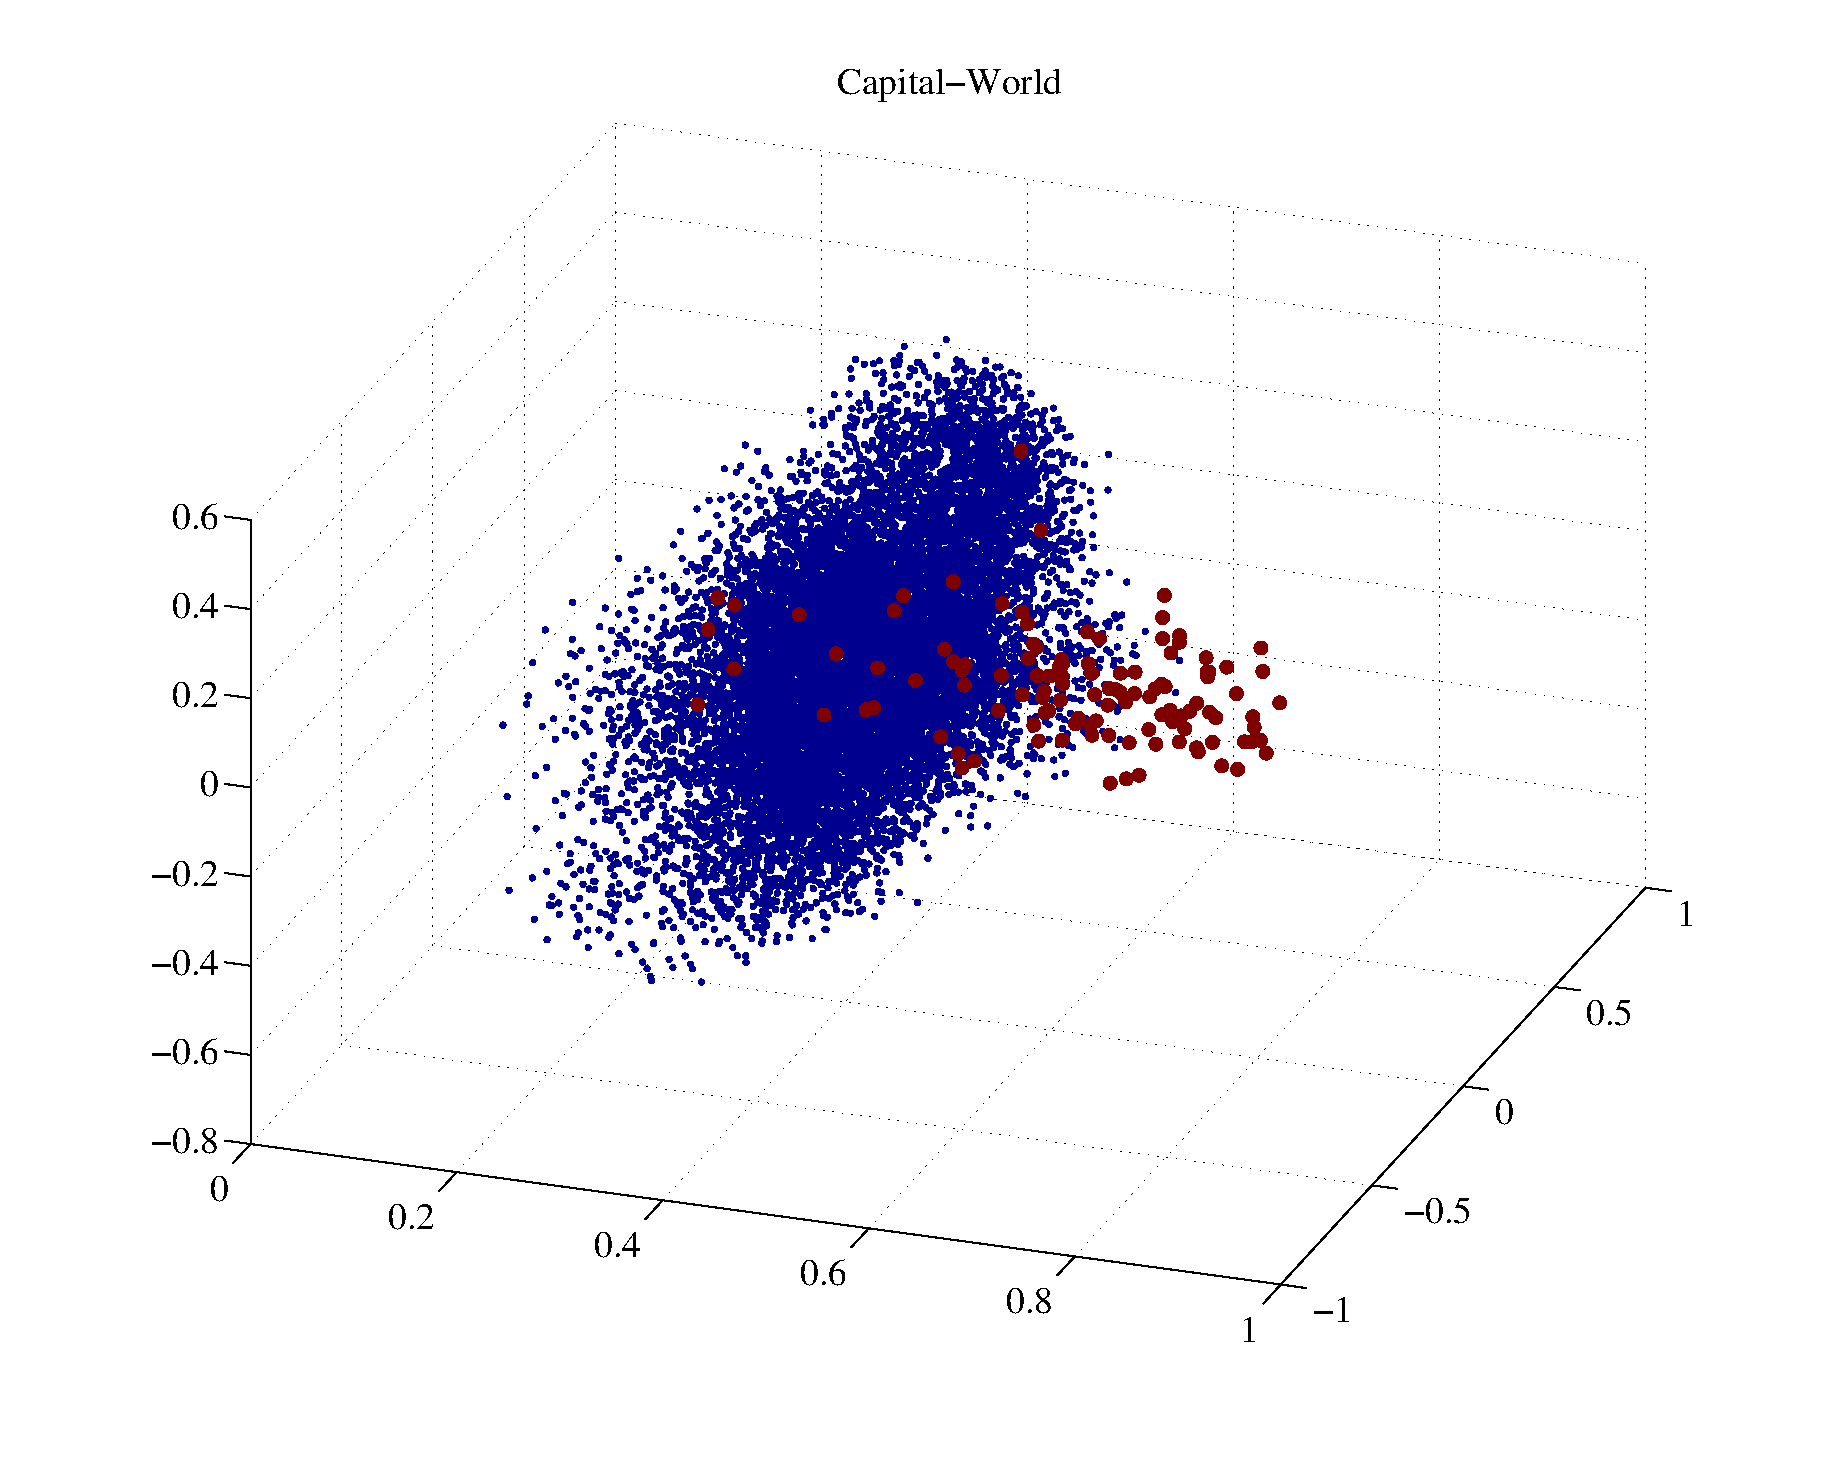
\includegraphics[width=.45\textwidth]{./images/capital_world.eps}
}
\subfigure[Nationality-Adjective]{
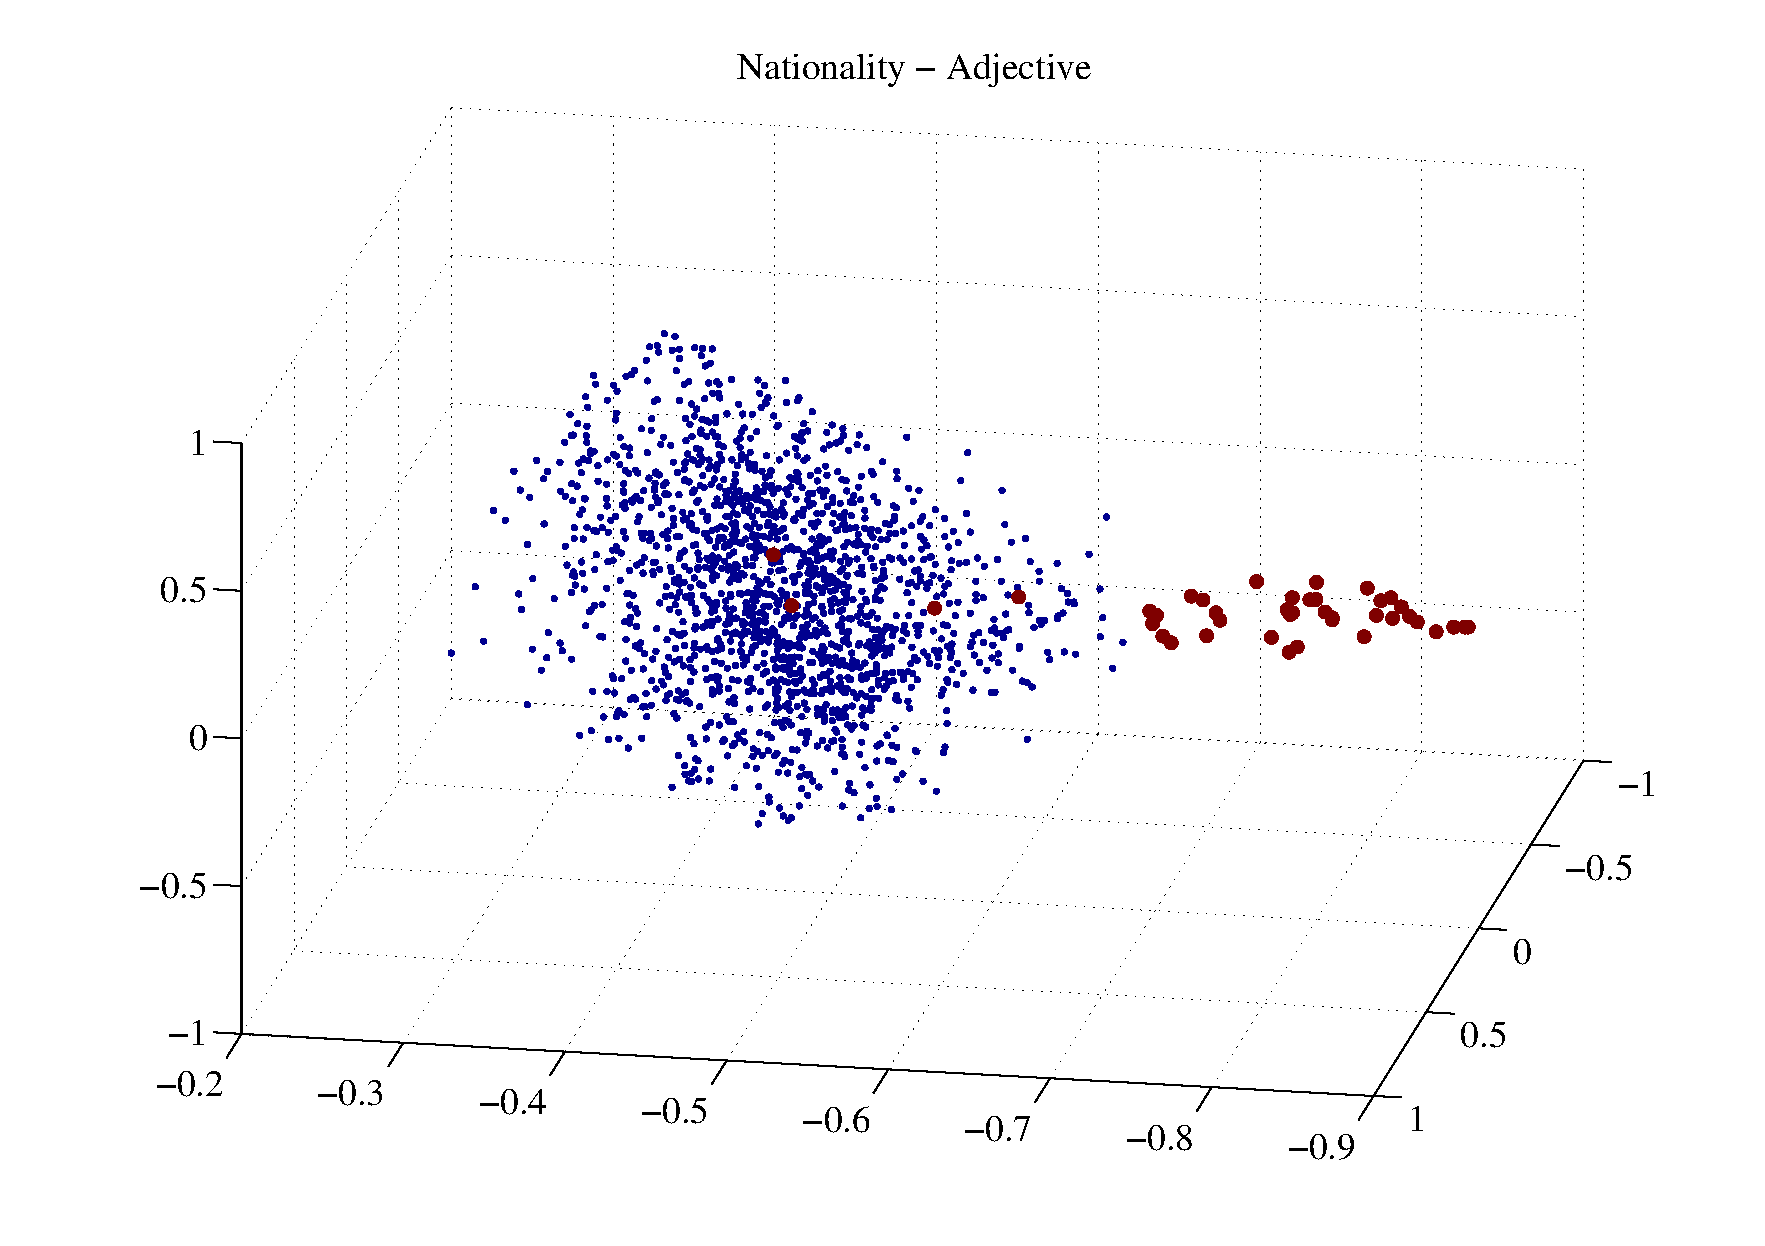
\includegraphics[width=.45\textwidth]{./images/nationality_adj.eps}
}

\subfigure[Plural-Vebs]{
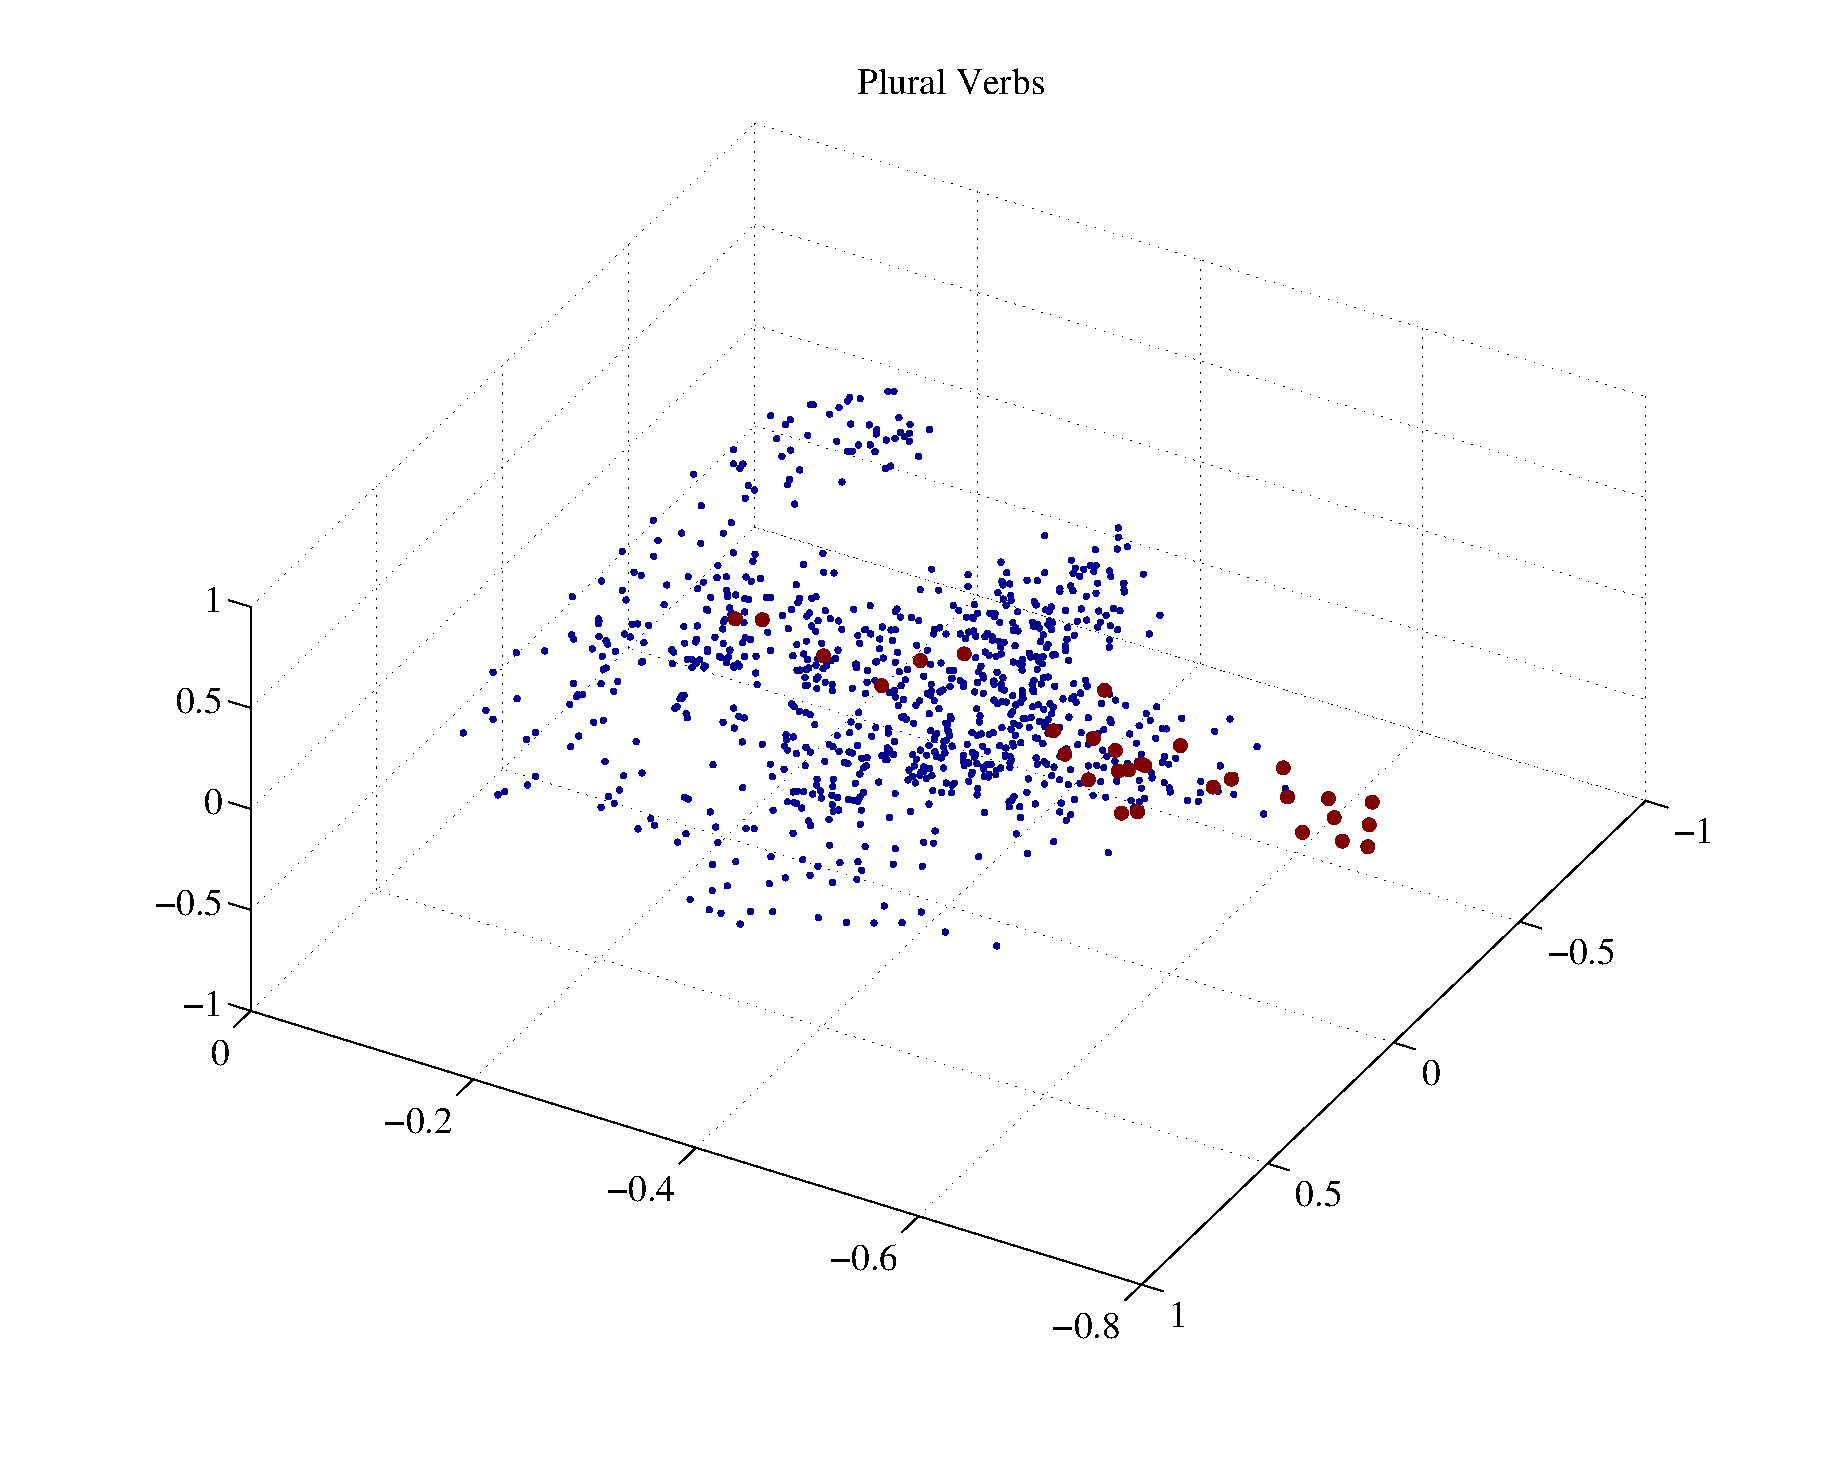
\includegraphics[width=.45\textwidth]{./images/plural_verbs.eps}
}
\caption{Projections of Vector Offsets for different categories of Word-Pairs}
\label{fig:offsetProj}
\end{figure}

\subsection{Low rank approximations of word vectors}
Ideally, we would like to be able to fit a variety of subspaces to all the word vectors. However, in practice the number of word vectors in our embedding space may be too large to afford running a subspace clustering algorithm on the entire set. To with this problem, we generate sets of words related by a high level concept and explore how well the word vectors associated with the set is approximated by a rank $k$ subspace, for varying $k$. If the set of vectors is well approximated by a rank $k$ subspace, for $k$ smaller than the original dimension of the space, then we can conclude the set of word vectors does in fact have linear low dimensional structure. Figure \ref{fig:svdOnClass} shows rank versus the $L2$ approximation error for word vectors in a variety of classes. As the figure shows, some classes are much more amenable to low rank approximations than others. This may partially be a product of our method generating related words (currently being done via a search of the WordNet hierarchy). 


\begin{figure}[t]
\centering
\includegraphics[width=.65\textwidth]{./images/svd_per_class.eps}
\caption{Rank vs. $L2$ error for different sets of word vectors}
\label{fig:svdOnClass}
\end{figure}

\nocite{*}
\bibliographystyle{splncs}
\bibliography{bibliography}

\end{document}
